\chapter{Background}
Starting my final year project at the Electronic Vision(s) group, I soon realized the diversity of their research. From the biological view of the human brain to electronic circuit laws further to machine learning algorithms, the required knowledge to work in this field is broad and manifold. In the next paragraphs, I will introduce the most important concepts and physical backgrounds upon which the presented research in this works is based on.

\section{The Biological Neuron}

It is estimated that the human brain contains around $10^11$ neurons. However, the cortex is not only made out of spiking neurons but also a high number of glia cells which provide energy and structural support to the neurons. The neuron itself can be divided into three different functional parts: dendrites, soma and axon (see figure -> ref to Figure). On a high level description the dendrites are responsible for managing all inputs from any neurons and transmit them further to the soma where the received information is processed. The output of the soma is then distributed via the axon to other neurons.  The input and output consists of short electrical pulses, spikes, which can either excite or inhibit the whole neuron membrane and thus lead to an in- or decrease of its electrical potential (\textit{membrane potential}). The link between two neurons is established by a synapse and usually a single neuron connects to around $10^4$ other ones. There is actually a small but physical gap between two connecting neurons called synapse cleft. When the \textit{presynaptic} neuron sends out a spike, a complex chain of reaction is triggered at the synaptic cleft, where various neurotransmitter will be released. Once a transmitter has connected with a corresponding receptor on the \textit{postsynaptic} side of the cleft, the receptor will activate ion channels which are responsible for raising or lowering the membrane potential of the postsynaptic neuron. By this the chemical reaction is converted back into an electrical signal.\\

\begin{figure}
	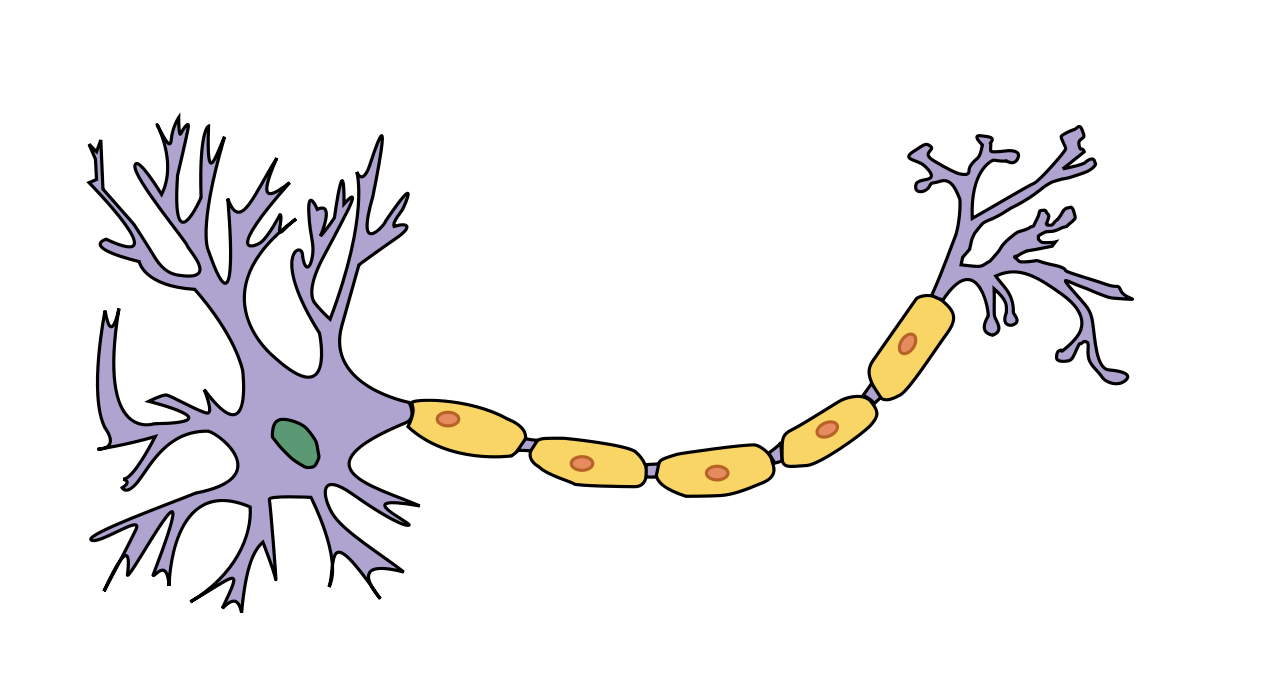
\includegraphics[width=\linewidth]{figures/neuron_model.png}
	\label{biosynapse}
	\caption{Schematics of a biological neuron: Dendrites, Membrane and Axon}
\end{figure}


In addition to the ion channels a neuron also contains ion pumps. These pumps restore the balance of the ion concentration in and outside of the membrane over time. The equilibrated state of the membrane potential is referred to as the \textit{resting potential}. Apart from an excited and a resting state, the neuron can also be \textit{refractory}. Once a spike has been fired, the neuron's membrane becomes hyperpolarized and the potential decrease even below the resting point. At the beginning of the refractory state it is impossible for the neuron to spike again. Due to the ongoing hyperpolarization also after this first period it remains hard but not impossible to send out a spike. The typical dynamics of the membrane are depicted in figure [ref to figure]. One should keep in mind that the shape of a spike doesn't carry any information.  The communication between neurons is rather encoded in the frequency and correct timing of exciting and inhibitory spikes. The various methods of spike coding are presented in section \ref{deeplearning}. 

\subsection{Leaky Integrate-and-Fire Model}

The input of a neuron is usually given by a number of input spikes from different presynaptic sources $j$ at various spike times $t^{(s)}$. This collection of spikes is called the input \textit{spike train} $S_j(t) = \sum_{t^{(s)}} \delta(t - t^{(s)})$ with $\delta$ the $\delta$-function. In a simplified model, the neuron's membrane $V_{\text{m}}$ sums over the synaptic input current $I_{\text{syn}}$ generated by the all input spike trains ("integrate"). As soon as there is no further input the neuron will slowly leak towards a resting potential $V_\text{leak}$. The dynamics of the membrane are defined by a single differential equation:
\begin{align}
C_{\text{m}} \frac{dV_{\text{m}}}{dt} &= -g_{\text{leak}} (V_{\text{m}} - V_{\text{leak}}) + I_{\text{syn}}.
\end{align}

The membrane's time constant $\tau_{\text{m}}$ is given by the ratio of the membrane capacitance ($C_{\text{m}}$) and the leakage conductance ($g_{\text{leak}}$): $\tau_{\text{m}} = \frac{C_{\text{m}}}{g_{\text{leak}}}$. 

Depending on the synapses weight $w_j$ each spike train has either an inhibitory or excitatory effect of different strength on the membrane. The synaptic current evolve as follows
 \begin{equation}
 I_{\text{syn}}(t) = \sum_j w_j \epsilon \ast S_j(t), 
 \end{equation}
where $\epsilon$ is either a single or double-exponential kernel. % or write it as theta (t - t_s) exp(...)
A "fire" mechanism is triggered at time $t_{\text{fire}}$ once the membrane crosses a certain threshold potential $\mathcal{\vartheta}$. 
\begin{align}
V_{\text{m}}(t_{\text{fire}}) &\ge \vartheta \Leftrightarrow \text{Neuron fires at time } t_{\text{fire}} \\
\end{align}
After releasing the response signal, the membrane is reset to $V_{\text{reset}}$ where it remains without any change for a refractory period of $\tau_{\text{ref}}$. 
\begin{align}
V_{\text{m}}(t) &= V_{\text{reset}} \quad \forall t \in (t_{\text{fire}}, t_{\text{fire}} + \tau_{\text{ref}}] 
\end{align}


The Leaky Integrate-and-Fire (LIF) model makes use of the fact that the shape of an input spike stays approximately the same. It was first described by Lapicque in 1907 [REF missing]. The model describes no spatial structures of the neurons. A LIF neuron is thus a point-like integrator that neglects any non-linear dynamics coming from strategically positioned connections to sources of excitatory or inhibitory spikes. Moreover a LIF neuron doesn't keep any memory of previous spikes after firing, since the membrane will always be reset to $V_{\text{reset}}$. These limitations make it impossible for the model to correctly describe neuronal behavior for repetitive firing. However, the main neuron dynamics are well described by the LIF neuron and it thus has been a popular choice for neuromorphic hardware [ref to BSS1?].\\

\begin{figure}
	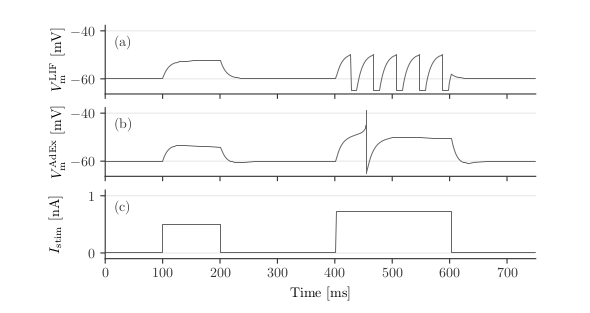
\includegraphics[width=\linewidth]{figures/LIFvsAdEx.png}
	\label{lifvsadex}
	\caption{Difference of membrane dynamics between a LIF and AdEx neuron, given the same synpatic input. Figure taken from Stradmann, 2019}
\end{figure}

The limitations of the LIF neuron led to a demand for a more sophisticated model, namely the Adaptive-Exponential Integrate-and-Fire short AdEx model. The two adaptations made are an additional adaptive current the allows the membrane to remember its previous state after firing and an exponential voltage feedback. Depending on the sign of the adaptive current, the neuron will either be stunted to fire again after it has sent out its first spike or it is engaged to keep on firing. In the example given in figure [ref to figure] the former is the case. The exponential voltage feedback on the other hand, enables the neuron to generate a proper fire response.\\

\subsection{Synaptic Plasticity (Learning)}
adapt weights and structure means learning

hebbian what wires together fire s together

LTP (long term potentiation) , STDP (spike timing dependent plasticity) , LTD (long term depression) -> and where are methods like superspike einzuordnen?




\section{Deep Learning}
\label{deeplearning}
The last decade was filled with inventions and technologies of machine learning nature. Among the many tools machine learning has provided to the scientific community, deep learning is one where many still struggle to grasp its mechanism and capabilities. However, it has become a useful and powerful tool to solve complex tasks. One approach is to understand such a task in terms of a hierarchy of concepts. Each concept is based upon a combination of simpler ones. Going done on a hypothetical ladder towards the easiest concept available, creates a deep structure with many layers. This is why it's called \textit{deep learning} . [Deeplearning Book, Intro]

The essential example of deep learning is the feedforward neural network or multilayer perceptron (MLP). In a feedforward network the information is passed from one layer to another. At each layer the input $\mathbf{x}$ is mapped to an output $\mathbf{y} = f(\mathbf{x, \theta})$ with a set of parameters $\mathbf{\theta}$ that can be trained in order to obtain the optimal result. These chain structures are inspired by biological neural networks and are thus often referred to as artificial neural networks (ANNs).\\

Given the task to identify a picture of cat, any computer will have a hard time to map the essential information of the camera's sensor data to the class \textit{cat}. An ANN solves the problem by learning how to describe the raw data in terms of simpler representations and essentially by combining these simpler representations into a meaningful solution in the last layer - the output layer. The first layer is called input layer and all other layers in between are named hidden layers, since they are usually not visible from the outside.\\

Neuromorphic hardware uses spikes to transmit data from one neuron to another and the mapping function is represented by the modeled neuron (e.g. the LIF neuron). In terms of deep learning, such networks are called spiking neural networks (SNNs). There are a number of different ways to use spikes for information encoding. \textbf{Rate coding} for instance uses a high number of spikes to establish a certain firing rate of the neuron. The information is not encoded in a single spike or the time interval between two spikes but in a number of spikes within a certain period defining the \textit{rate}. \textbf{Temporal coding} on the other hand focuses on the interspike interval (ISI). This type of coding is more exposed to noise but for some applications it might be simply too slow to establish a certain fire rate first. The ISI on the other can be adapted quickly. When only a small set of all available neurons is used to describe an input pattern, its called \textbf{sparse coding}.\\

The different types of neural coding require each an adapted training method. Rate coding can be treated similar to ANNs and thus classical training methods such as gradient descent will work just fine. However, for temporal or sparse coding the gradient descent approach doesn't work since the binary nature of spikes make the neurons output non-differentiable. In 2017 Friedemann Zenke has proposed with SuperSpike a surrogate gradient descent implementation for SNNs that successfully overcomes this issues. 

\subsection{Training Methods for ANNs}
\label{trainingANN}

The learning process of a neural network can be divided into a forward and backward pass. During the forward pass the output value of each node in the network is evaluated. The backward pass computes in which direction the networks parameters $\mathbf{\theta}$ need to be changed so that they minimize a given loss function $\mathcal{L}(\mathbf{\theta})$.

\subsubsection{Forward Pass}
The activation $\mathbf{a}$ of a layer is given by the weighted input $\mathbf{x}$ with a weight matrix $W$ plus a bias term $\mathbf{b}$. The bias term is a vital parameter which allows the network to shift the dynamic range of a single neuron. 
\begin{align}
\mathbf{a} = W \, \mathbf{x} + \mathbf{b} \\
\end{align}
 
The output $\mathbf{y}$ of the layer is the result of the transfer function $\phi$ and which is chosen to be of sigmoidal shape. The exact shape of the transfer function is not of high importance, as long as at it is non-linear. In combination with a cross-entropy loss function the choice of a sigmoid becomes convenient when performing the backward pass.

\begin{equation}
\mathbf{y} = \phi(\mathbf{a}).
\end{equation}

The same principle is applied to all other layers in a forward direction, i.e. the result of the previous layer is the input for the current layer. The weight matrix $W^{\text{(l)}}$ connecting layer $l$ with the predecessor has the appropriate shape to fit the number of input nodes (i.e. the number of nodes in the previous layer) and the number of nodes in the current layer. In figure [ref to 1 layer structure].

\subsubsection{Gradient Descent (Backward Pass)}

Most training approaches for neural networks involve optimizing a loss function $\loss(\mathbf{\theta})$ by changing the networks parameters $\mathbf{\theta}$ in the correct direction. This can be achieved by moving in the along the negative gradient of the $\loss$. The new set of parameters $\mathbf{\theta'}$ is then given by [compare deep learning book ch 4]
\begin{equation}
\mathbf{\theta'} = \mathbf{\theta} - \eta \, \nabla\loss(\mathbf{\theta}).
\end{equation}
whereby $\eta$, the learning rate, defines how \textit{fast} an update is applied.\\

As an example the update of the weight matrices $\delta W_{\text{(o)}}$ is computed. Other parameter updates, such as the update of the bias are done in analogy to the weights. First it necessary to know what the loss function looks like. This is why the computation starts from the end of the layer structure, the output layer. The derivative of the sigmoid yields $\frac{\partial \mathbf{y}}{\partial \mathbf{a}} = \frac{\partial \phi(\mathbf{a})}{\partial \mathbf{a}} = \phi (1 - \phi)$ and the derivative of the imposed a cross-entropy loss is given by
\begin{align}
\frac{\partial\mathcal{L}}{\partial \mathbf{y}} = 
- \frac{\hat{\mathbf{y}}}{\mathbf{y}} + 
\frac{1 - \hat{\mathbf{y}}}{1 - \mathbf{y}}
\end{align}
with $\mathbf{y}$ the output and $\hat{\mathbf{y}}$ the target output. The error $\mathbf{e} = \hat{\mathbf{y}} - \mathbf{y}$ can then be rewritten in terms of the partial gradients
\begin{equation}
\Rightarrow \quad \frac{\partial\mathcal{L}}{\partial \mathbf{a}} =
\frac{\partial\mathcal{L}}{\partial \mathbf{y}} 
\; \frac{\partial \mathbf{y}}{\partial \mathbf{a}} =
\hat{\mathbf{y}} - \mathbf{y} = \mathbf{e}.
\end{equation}
Now the weight update $\delta W^{\text{(o)}}$ for the output layer yields 
\begin{align}
\delta W^{\text{(o)}} =& - \eta \frac{\partial \mathcal{L}}{\partial W} 
= - \eta \;
\frac{\partial\mathcal{L}}{\partial \mathbf{y}} \;
\frac{\partial \mathbf{a}}{\partial W}
= - \eta \, (\mathbf{e} \cdot \mathbf{x}^T),
\end{align}
with $\mathbf{x}$ being the input of the output layer, thus the output of the hidden layer.

The result for the hidden layer computes similarly. Again we look at the gradient of the loss function and find
\begin{align}
\frac{\partial\mathcal{L}}{\partial \mathbf{a}} &= \left(W^{\text{(o)}T} \cdot \mathbf{e}\right) \;
\frac{\partial \mathbf{y} }{\partial \mathbf{a}}\\
\Rightarrow \quad \delta W^{\text{(h)}} &= - \eta \;
\left(W^{\text{(o)}T} \cdot \mathbf{e}\right) \;
\frac{\partial \mathbf{y} }{\partial \mathbf{a}} \;
\mathbf{x}^T,
\end{align}
Where $W^{\text{(o)}T}$ denotes the transpose of the weights of the output layer, i.e. the weights connecting the output layer to the hidden layer in backward direction. The backward propagation of the error is name giving and thus it is often referred to as \textit{back propagation}. Despite the great performance for many deep learning tasks, the biological plausibility of propagating the error signal backward in time has been questioned ever since. 

In 2016 a simple but effective adjustment has been proposed by Lilicrap et al. named \textit{feedback alignment}: Instead of the transpose of the weight matrix a fixed randomized one is chosen. Apart from providing more biological plausibility it also reduces the computational costs of plasticity rule. Compared to the back propagation the updates only change in the hidden layer:

\begin{equation}
\delta W^{\text{(h)}} = - \eta \;
(B \cdot \mathbf{e}) \;
\frac{\partial \mathbf{y}}{\partial \mathbf{a}} \;
\mathbf{x}^T,
\end{equation}
with B being a random matrix with corresponding dimensions.

\subsubsection{Gradient Descent for SNNs}

Spikes can encode information in various ways. One of them is rate coding, where a certain fire rate is established and the rate itself contains the information. Other then for sparse or spike time dependent coding, the information of a single spike is not relevant. The transfer function of the neuron contains still an activation jump. At a certain input rate the neuron will suddenly start to fire. This can be smoothen out by setting the leak and threshold potential close to each other and by adding Poisson distributed noise spikes. In combination this will establish a certain equilibrium fire rate given there is no further input. Now, by applying inhibitory input the fire rate will go down. Excitatory input causes the opposite.

The above described method turns a SNN almost into an ANN. However, The forward pass is still not performed perfectly by a powerful GPU but by a noisy and power-efficient analog core. Noise is essential for learning algorithms to perform and is often artificially injected for ANNs. This is not necessary for the BSS2 platform. In the experiment section, gradient descent with feedback alignment is conducted on the HICANN-DLSv2.


\subsection{Novel Training Methods for SNNs}


Until now, only few people have successfully trained SNNs with hidden units. The main issue arises from the non-differentiable dynamics of spikes. A promising approach was proposed by Friedemann Zenke in 2017 with SuperSpike. Similar to the training ANNs the learning process can be split up into forward and backward pass. 

\subsubsection*{Forward Pass}
The forward pass only changes slightly compared to ANNs. Instead of a continuous input and output one speaks of presynaptic spike train $S_j$ and a postsynaptic spike train $S_i$. Note that the choice of the index $j$ and $i$ indicate if, from the perspective of a neuron, the spike is of presynaptic or postsynaptic origin. The transfer function $\phi$ is replaced by the dynamics of the LIF neuron.

%Todo: "surrogate gradient" is not really introduced but just used -> fix this
%Todo: spike train formalism (maybe in biological part with synapses, etc. ), presynaptic/postsynpatic 
%Todo: axonal delay is not considered for the application of the hardware
%Todo: auxilary function: threshold! -> f(x) = x/(1 + |x|) and f'(x) (1 + |x|)-2 => $\sigma'(U_i) = (1+|U_i - \vartheta|)^{-2}$

\subsubsection*{Backward pass}

As stated in section \ref{trainingANN}, training a neural network requires the optimization of a certain loss function $\mathcal{L(\mathbf{\theta)}}$ that depends on the network's parameters $\mathbf{\theta}$, i.e. the synpatic weights $w_{ij}$. In the SuperSpike formalism the von Rossum distance of a target spike train $\hat{S}_i$ and the output spike train $S_i$ is chosen (cf. van Rossum 2001, Gardner and Grüning, 2016),
\begin{equation}
\label{vonrossumdistance}
\mathcal{L} = \frac{1}{2} \int^t_{-\infty}dt' \left[\left(\alpha \ast \hat{S}_i - \alpha \ast S_i \right)(t')\right]^2
\end{equation}
where $\alpha$ is a smooth double exponential convolution kernel. The computation of the gradient for \ref{vonrossumdistance} with respect to $\mathbf{\theta}$ requires the derivative of a spike train $\nicefrac{\partial{S_i}}{\partial{w_{ij}}}$ which is undefined for the time of a spike. 

SuperSpike circumvents this issue by rendering the spike train with a smooth auxiliary function $\sigma(V)$ of the membrane potential $V$ and thus the ill defined gradient of the spike train can be replaced by a surrogate derivative $\sigma'(V)$
\begin{equation}
\frac{\partial S_i}{\partial w_{ij}} \quad \rightarrow \quad \sigma'(V_i)\frac{\partial V_i}{\partial w_{ij}}.
\end{equation}

The choice of the auxiliary function $\sigma$ the therefore implied surrogate derivatives is to a certain degree free. SuperSpike suggest a deterministic approach with the negative side of a fast sigmoid $\sigma(V) = \frac{V - \vartheta}{1 + |V - \vartheta|}$. The surrogate partial derivative yields $\sigma'(V) = \left(1 + |V - \vartheta|\right)^{-2}$. Another common choices are pieces-wise linear or exponential approaches.

At a first glance, it appears that the problem has just been moved to computing the partial gradient of the membrane potential instead. When the potential $V_i$ is formulated as a spike response model for LIF neuron (Gerstner et al., 2014) it again depends on the output spike train $S_i$. However, under the assumption of a low output rate the gradient can be approximated by $\frac{\partial U_i}{\partial w_{ij}} \approx (\epsilon \ast S_j)$ with $\epsilon$ another double-exponential kernel corresponding to the shape of a spike. Plugging in the approximation and the formulation of the gradient as a surrogate gradient yields

\begin{equation}
\frac{\partial w_{ij}}{\partial t} = \eta \int_{-\infty}^{t} dt
\underbrace{\left(\alpha \ast (\hat{S}_i - S_i)\right)}_{= e^{(o)}_k \; \text{(Error)}} 
\; \alpha \ast 
\Big(\underbrace{\sigma'(U_i)}_{\text{Pre}} 
\underbrace{\left(\epsilon \ast S_j\right)}_{\text{Post}}\Big)
\end{equation}
with $\eta$ the learning rate. The formulation for the hidden layer is similar with the only exception of how the error is calculated. Inspired from the popular backpropgation method the error signal of the $i \text{-th}$ hidden unit $e^{(h)}_i$ is propagate backwards as a weighted sum over the all output error signal $e^{(h)}_i = \sum_{k} w_{ik} e^{(o)}_k$ with $w_{ik}$ the feed forward weights between the hidden and the output layer. A feedback alignment oriented approach with random weights is also possible. This formalism can be easily adapted for multiple hidden layers too.


%ToDo: Literatur Book zu Deep Learning (siehe downloads UniRechner)
%
%Überleitung zu rate coding vs sparse coding (maybe read again SuperSpike17/19 first))
%A spiking neural network (SNN) offers many advantages compared to a classical artifical neural network (ANN). On of the major differences is that sparse coding allows the user to compress a lot of information into a single spike. Also not spiking at a sppecifencodes information.  This efficient way of transporting information makes SNNs a contender for any energy sensitive form of computing. More importantly it also opens up the doors to understanding spike-based computing better and thus also the way the human brain works.

\subsection{Neuromorphic Hardware}

Biological inspired computing is as popular as it has never been before. IBM started to work on \textit{TrueNorth} in 2008, Intel presented the \textit{Loihi} chip in 2018 and Google started selling the \textit{Coral} dev-board in 2019. Among these industry project, several academic projects have started as well. The EU's Human Brain Project (HBP) funds two serious contenders: \textit{SpiNNaker}, a digital based neuromorphic supercomputer and \textit{BrainScaleS} (BSS) a mixed-signal accelarated emulation for spiking neural networks. The later has its early beginnings back in the late 80s.

The BSS2 system, the most recent version of the BrainScaleS platform, is based upon a physical implementation of neurons and synapses which is manufactured by the Taiwan Semiconductor Manufacturing Company (TSMC) using a $65 \si{nm}$ low-power and low-leakage CMOS technology. The BSS2 successor BSS1 used already a High Input Count Analog Neural Network (HICANN) chip. The new version of the chip contains 512 AdEx neuron circuits, 256 possible synpatic connections per neuron, two plasticity processing units and on chip routing. In accordance with the predecessor's name, it is called HICANN with Digital Learning System and Hagen eXtensions (HICANN-X). The new features have been implemented step by step on smaller prototype system. One of them is the HICANN-DLSv2. Instead of the AdEx neuron model only 32 LIF neurons are featured, but a 32x32 synpase array allows an all to all connectivity. Besides the Hagen eXtension, the main features of the BSS2 system have been implemented on the HICANN-DLSv2. In the following section the individual parts of the chip are discussed. The concept and functionality of each part stays the same throughout the different chip version of the BSS2 system.

The experiments conducted within this thesis use either the HICANN-X or the DLSv2 chip.
%in various \textit{application-specific integrated circuits} (ASICs).
%refs: ibm http://www.research.ibm.com/articles/brain-chip.shtml
% coral board:
% Loihi:

\begin{figure}
	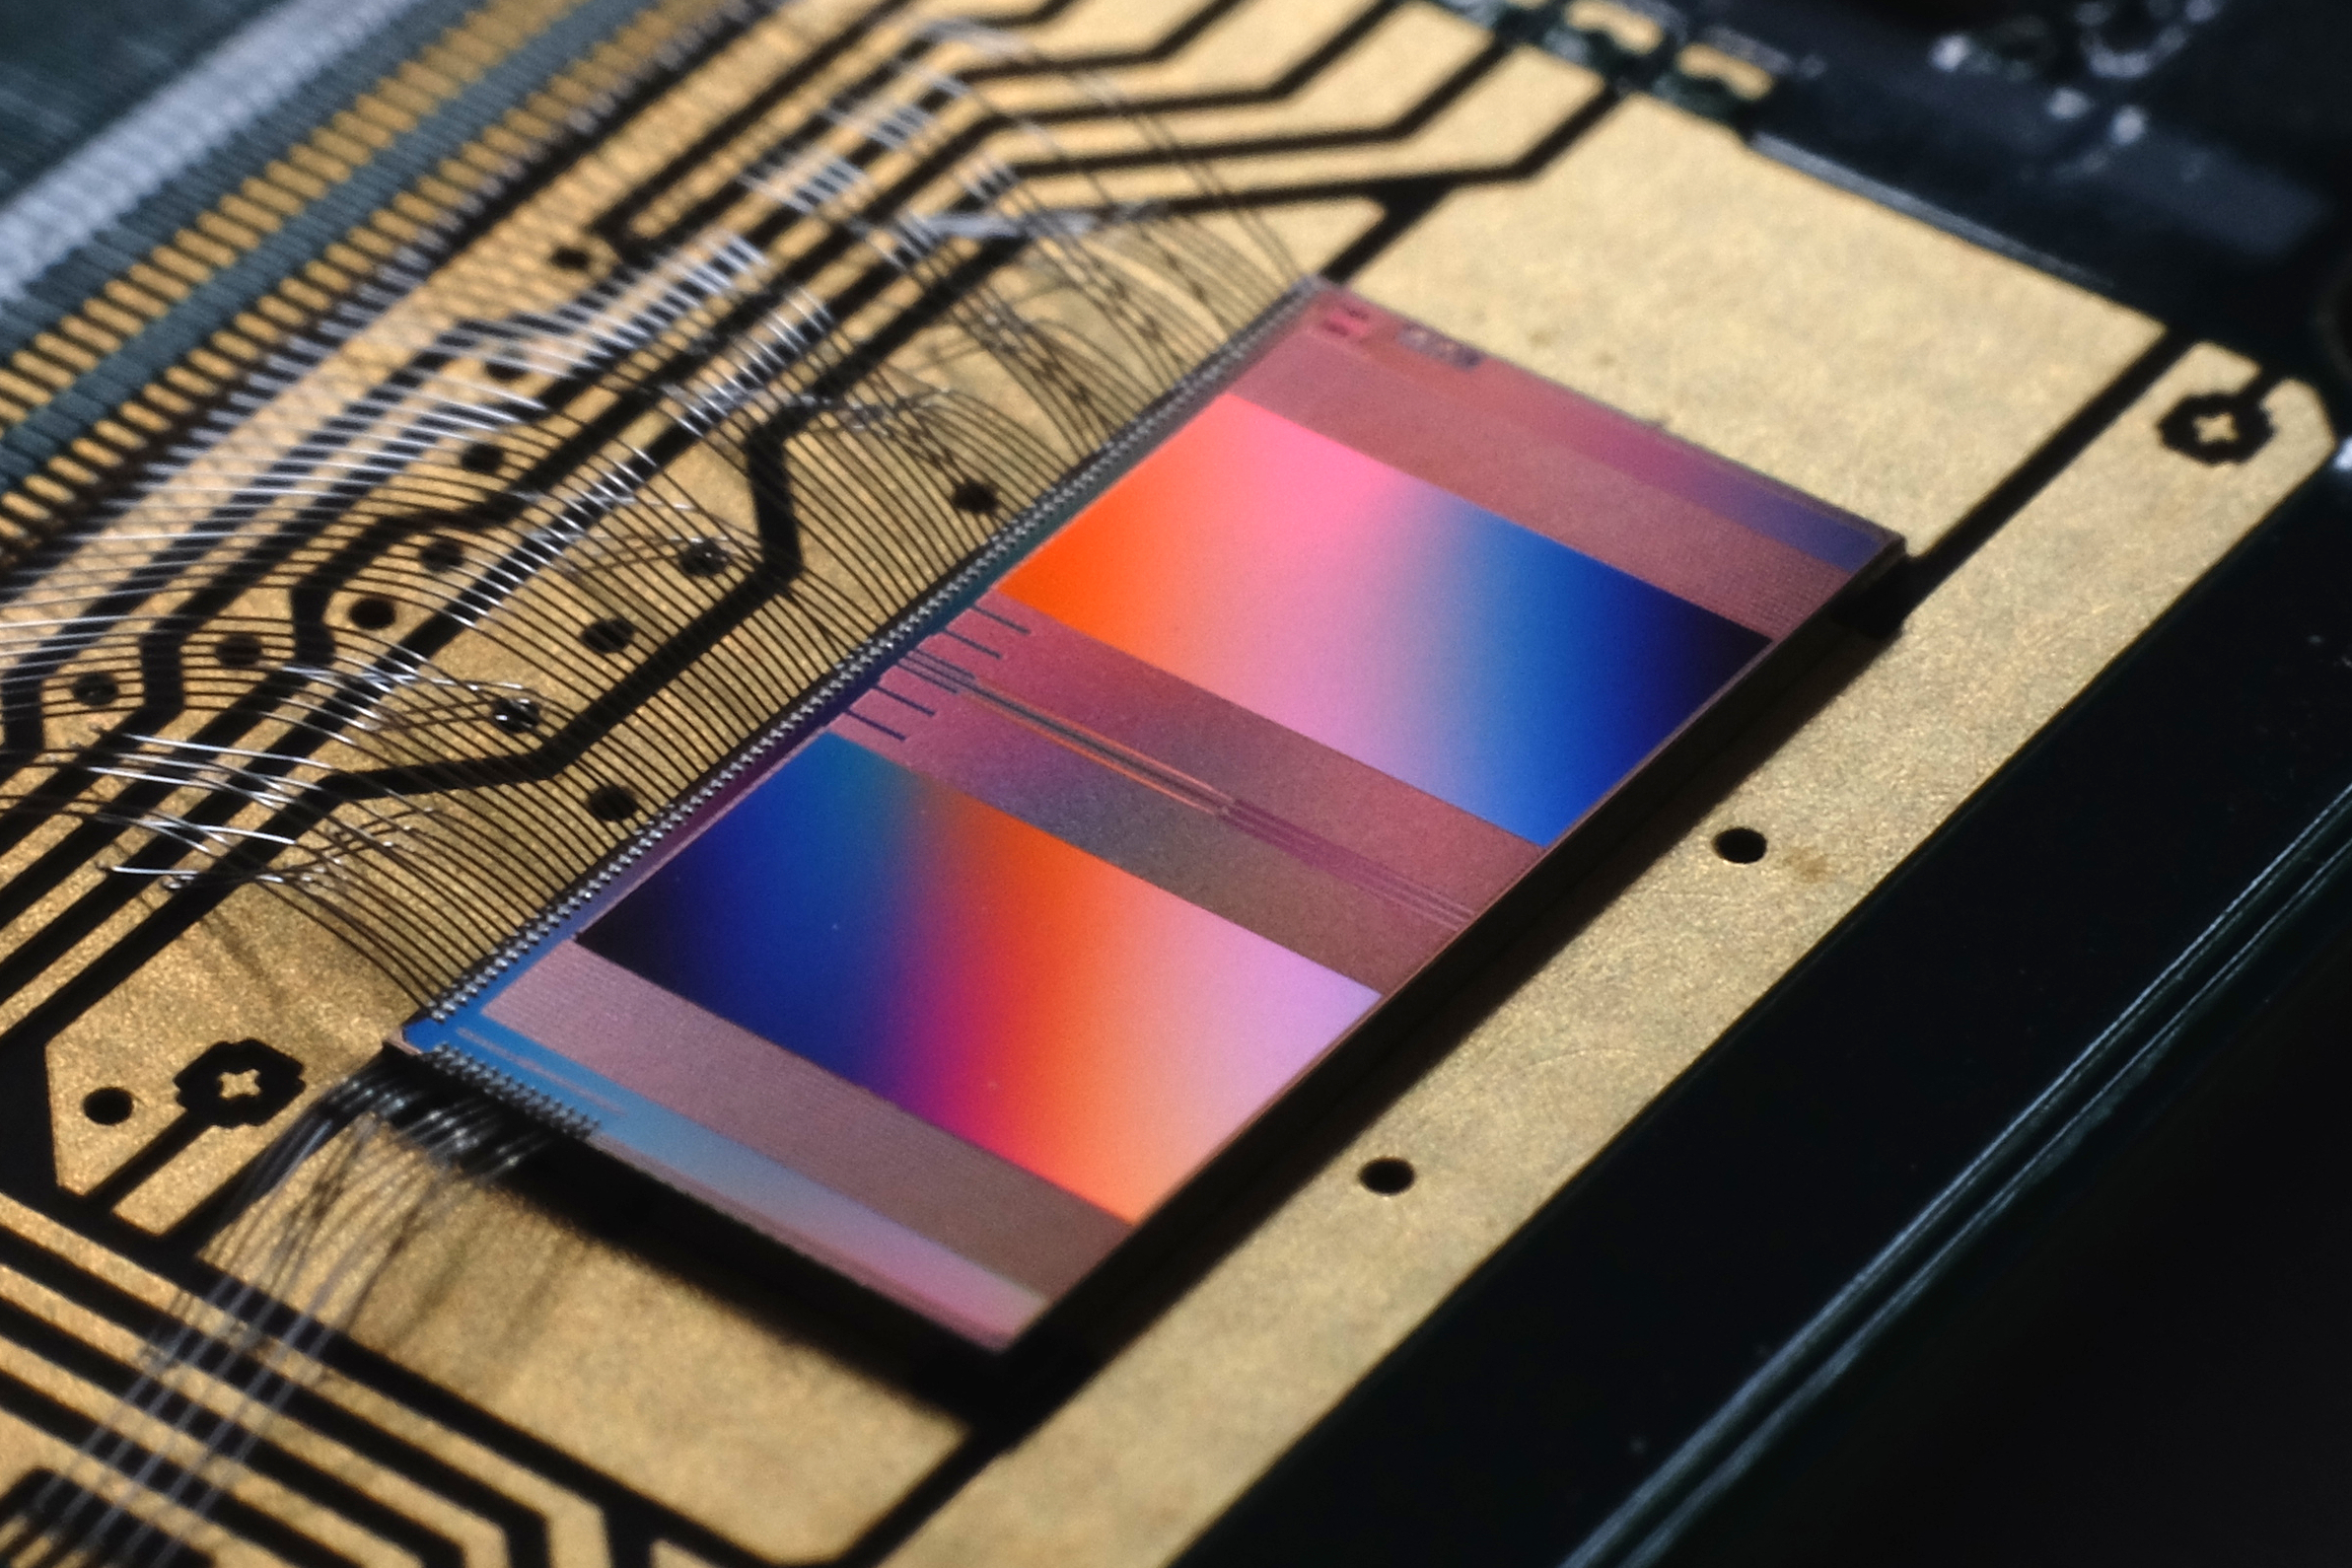
\includegraphics[width=\linewidth]{figures/HXcloseup.JPG}
	\label{hxcloseup}
	\caption{Close-up of the bonded analog core of the HICANN-X chip. Picture taken by Müller, 2020}
\end{figure}

\subsubsection{Architecture of BSS2}

The design of the HICANN-X chip can be divided into an analogue and digital core (c.f. figure \ref{HXstructure}). The communication with an external host is streamed out to the controlling Field Programmable Gate Array (FPGA). The existing FPGA solution developed for BSS1 was simply transfered to BSS2.

\begin{figure}
	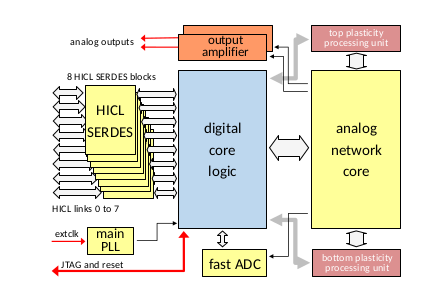
\includegraphics{figures/HXstructure.png}
	\label{hxstructure}
	\caption{Overview of the architecture of the HICANN-X chip. Figure taken from (Schemmel,2017)}
\end{figure}

\subsubsection*{Analogue and Digital Core}
The analogue core implements the neuron dynamics. On the DLSv2 a current based LIF neuron model with a total of 32 neurons is used (Aamir, Müller et al. 2016, ...). The dynamics of an \textit{in-silico} neuron have a temporal speed-up factor of 1000 compared to its \textit{in-vivo} counterpart. This acceleration is made possible by the supra-threshold dynamics of CMOS transistors. The biological time constants of neurons and synapses are usually in the order of 10 to 100 milliseconds. The HICANN-X contains 512 AdEx neurons. AdEx is short for a LIF model extension with an adaptive current and an exponential voltage feedback. The analog model parameters in both chips are tunable by setting bias currents over an 10 bit Digital to Analog Converter (DAC). (Hock et al., 2013) Each neuron can be controlled and adjusted individually. The 8bit spike counter of the DLSv2 (one per neuron) has been upgraded to a 10 bit counter in the HICANN-X. 

The synaptic input is mapped by an $512 \times 256$ synapse array. Each synapse has a 16 bit local Static Random Access Memory (SRAM) to store weight and information about the presynaptic connections. In addition, two correlation sensors per synapse (causal and anti-causal) record STDP traces and store them in dedicated capacitors. These analog observables can then be accessed by a Plasticity Processing Units (PPU) via an Analog to Digital Converter (ADC). The readout is performed per row and thus a total of 1024 channels (one channel per correlation sensor per synapse) is accessed by the \textit{Correlation} ADC (CADC). The CADC can also be used to access further observables such as the membrane potential. This feature has not been available on the earlier revision and opens up new possibilities for plasticity rules. A highly accelerated analog system requires a fast computation of any plasticity rule. To provide sufficient computational power, the chip is equipped with two asynchronous Single Instruction Multiple Data (SIMD) PPUs. The PPU has vectorial access to the synapse array as well as to the results of the CDAC.   

As an additional debugging and observation tool, a fast ADC (MADC) can be accessed from the digital core to readout any available analog observables.

Apart from the spike counters, the digital neuron backend registers any spiking event. Such an event may also come from one of the noise generators or PPUs as well as from an external source. Once a spike has been registered in the digital neuron backend, it is routed back into the synapse array accordingly. 

\subsubsection{Communication}
The link between chip and external host is established through eight serial Low Voltage Differential Signaling (LVDS) links that are accessed by an FPGA. This interface handles all read/write instructions to any SRAM on chip and manages spike event data in both directions. The FPGA grants access for the PPU to greater memory storages than the one provided on-chip. Access to large training datasets is vital for most learning tasks.

%The communication for DLSv2 is slightly adapted. 
